\section{Siliceno}


\begin{frame}{Siliceno}

    \textbf{Párametro de red}

    \begin{figure}[H]
        \centering
        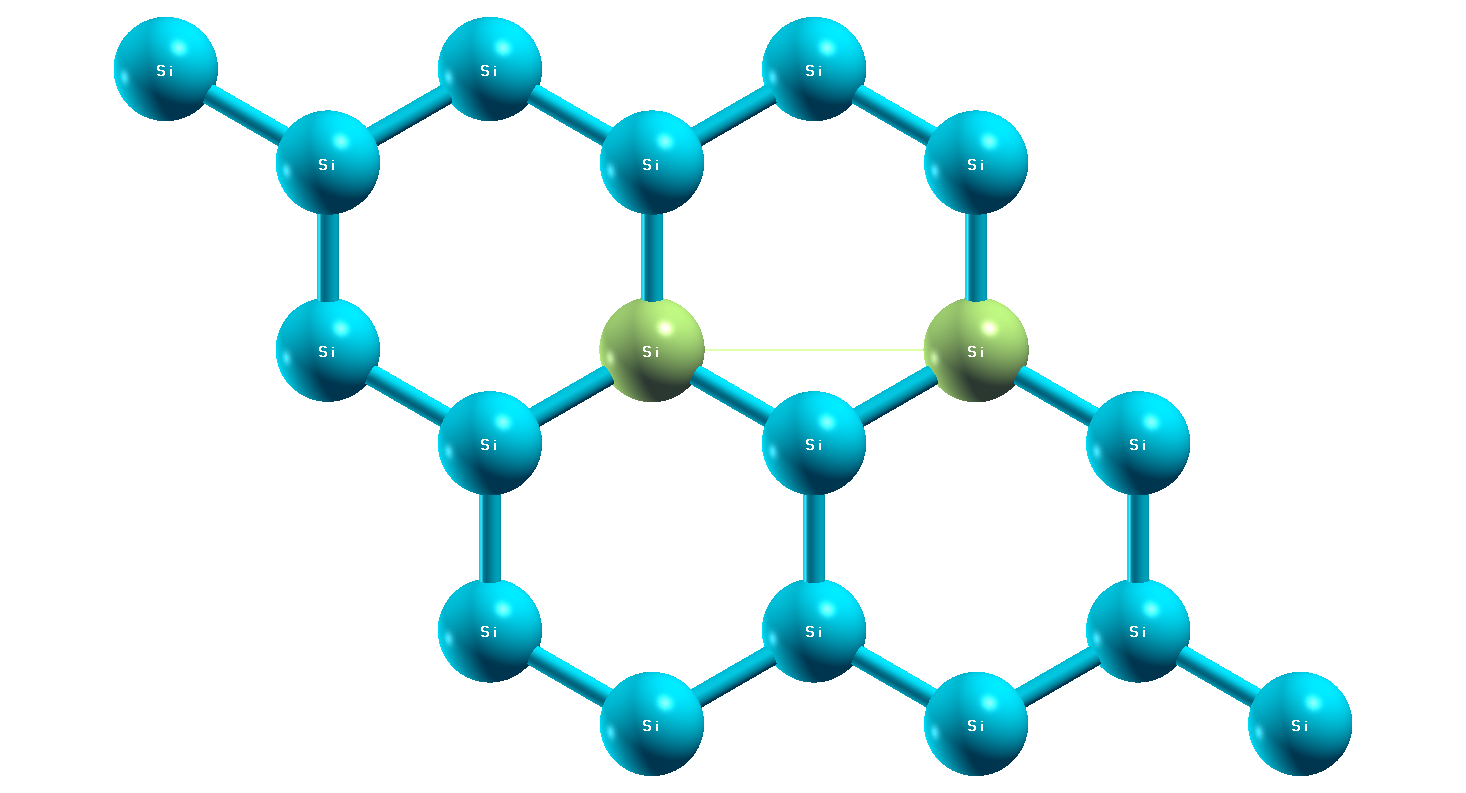
\includegraphics[scale=0.2]{images_siliceno/longitud_enlace_3_8600_amstrongs.png}
        \caption{La longitud del enlace mostrado es de 3.8600 amstrongs.}
    \end{figure}
\end{frame}


\begin{frame}

    \textbf{Estructura electrónica de bandas (sin considerar el spin)}

    \begin{figure}[H]
        \centering
        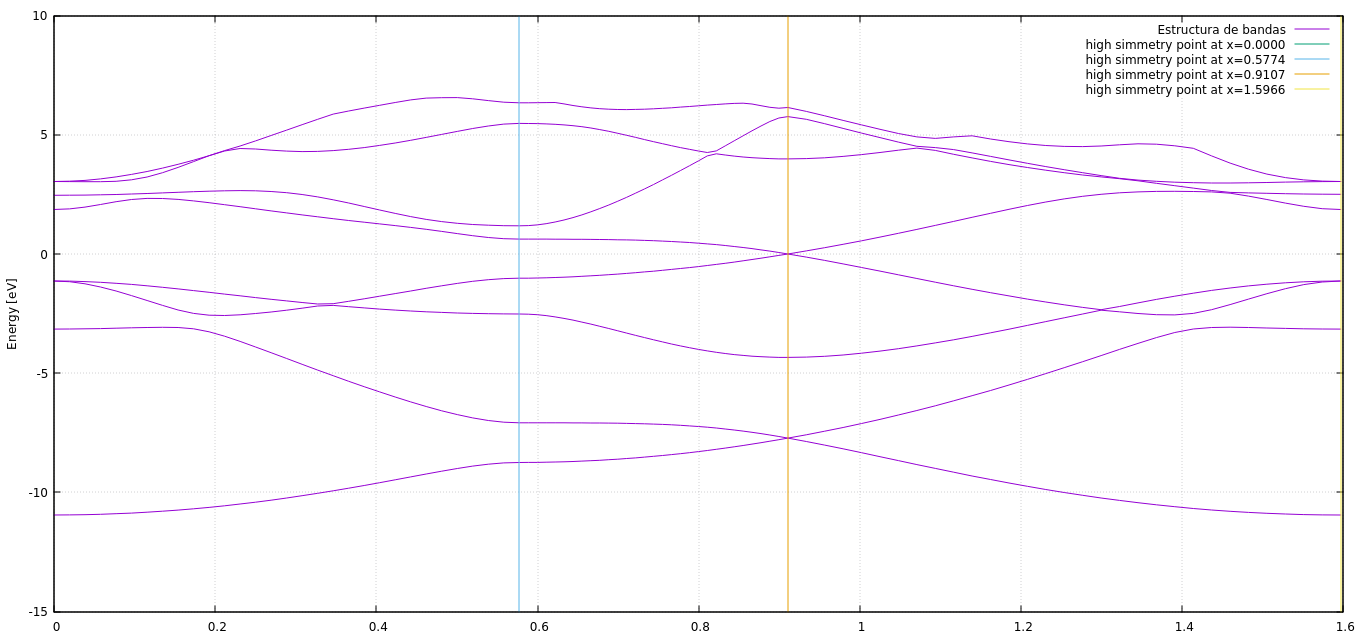
\includegraphics[scale=0.34]{images_siliceno/bands_structure.png}
        \caption{Estructura de bandas del Siliceno.}
    \end{figure}
\end{frame}

\begin{frame}
    \begin{figure}[H]
        \centering
        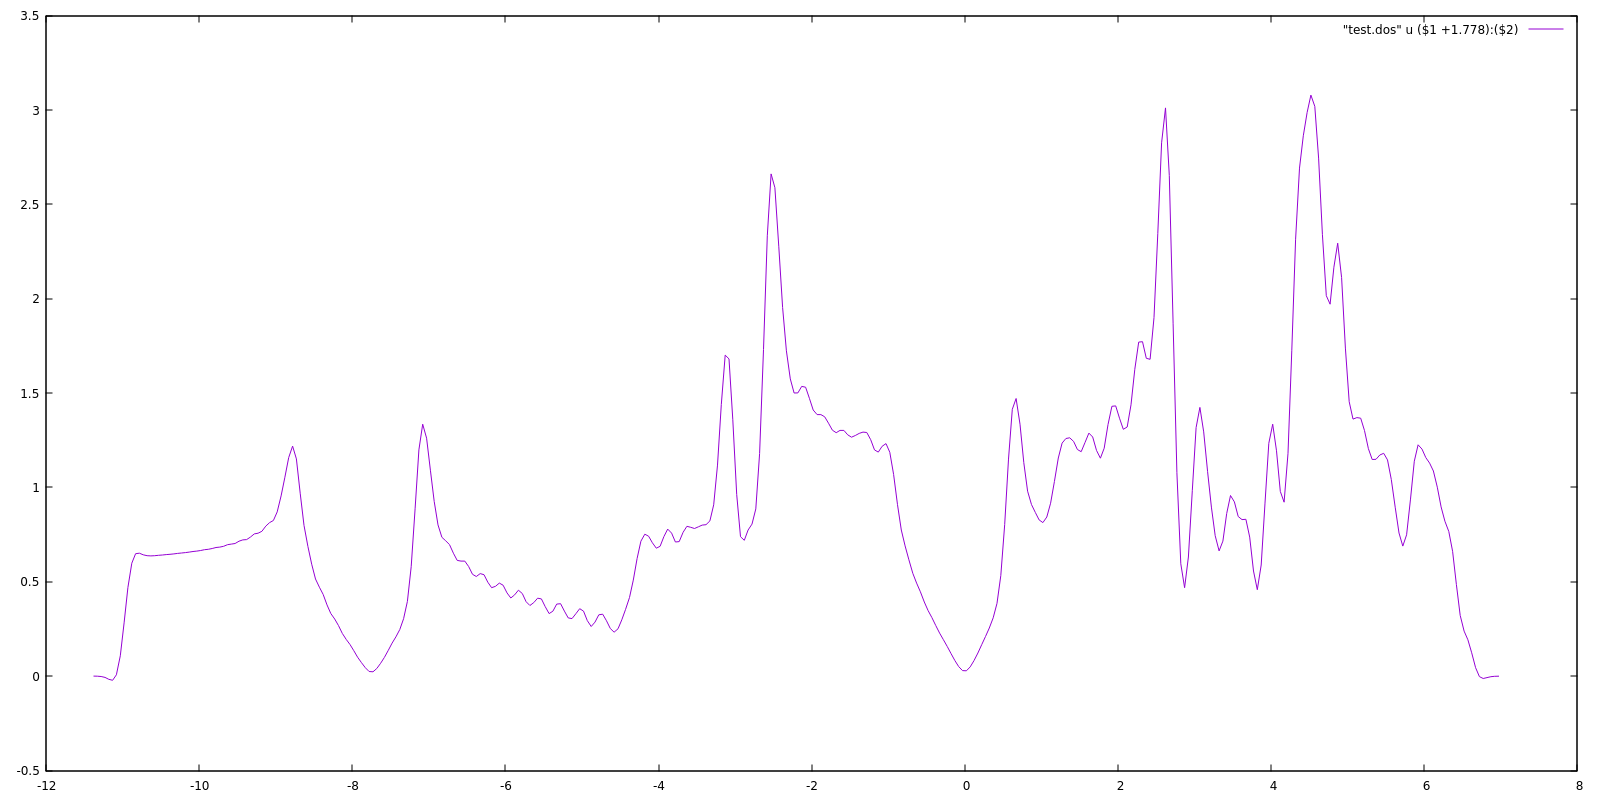
\includegraphics[scale=0.25]{images_siliceno/plot_sin_spin.png}
        \caption{Gráfica que nos muestra la densidad de estados del siliceno, sin considerar el spin.}
    \end{figure}
\end{frame}

\begin{frame}
    \begin{figure}[H]
        \centering
        \includegraphics[scale=0.3]{images_siliceno/siliceno_energía_orbitales_up_sin_spin.png}
        \caption{Gráfica que nos muestra la densidad de estados en los orbitales del siliceno, sin considerar el spin [UP].}
    \end{figure}
\end{frame}

\begin{frame}
    \begin{figure}[H]
        \centering
        \includegraphics[scale=0.3]{images_siliceno/siliceno_energía_orbitales_down_sin_spin.png}
        \caption{Gráfica que nos muestra la densidad de estados en los orbitales del siliceno, sin considerar el spin [DOWN].}
    \end{figure}
\end{frame}


\begin{frame}

    \textbf{Estructura electrónica de bandas (considerando el spin)}

    \begin{figure}[H]
        \centering
        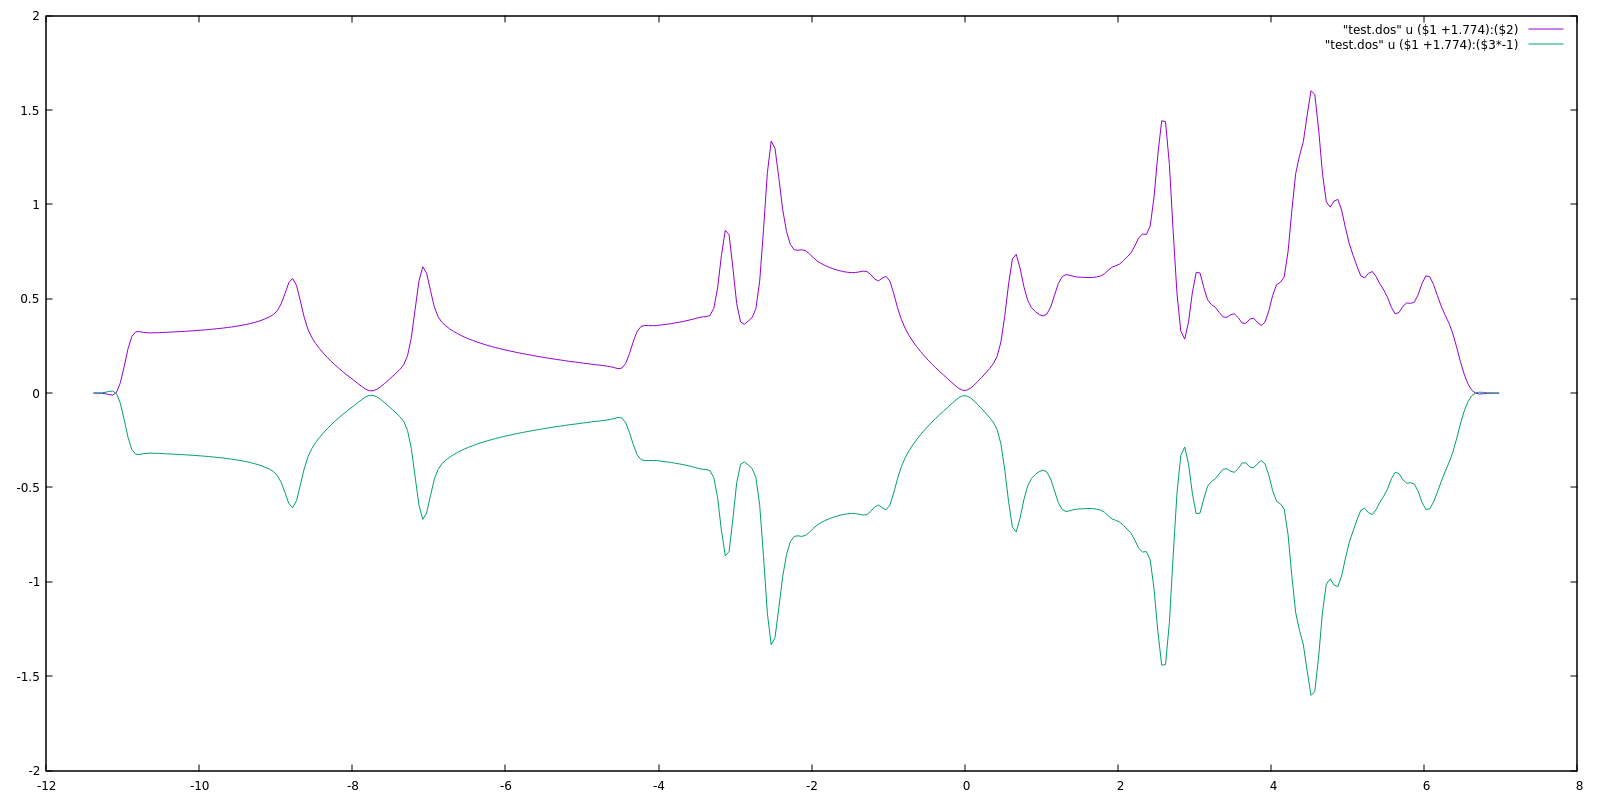
\includegraphics[scale=0.25]{images_siliceno/densidad_estados_con_spin.png}
        \caption{Gráfica que nos muestra la densidad de estados del siliceno, considerando el spin.}
    \end{figure}
    
\end{frame}

\begin{frame}
    \begin{figure}[H]
        \centering
        \includegraphics[scale=0.3]{images_siliceno/silicio_energía_orbitales_up.png}
        \caption{Gráfica que nos muestra la densidad de estados en los orbitales del siliceno, considerando el spin [UP].}
    \end{figure}
\end{frame}

\begin{frame}
    \begin{figure}[H]
        \centering
        \includegraphics[scale=0.3]{images_siliceno/siliceno_energía_orbitales_down.png}
        \caption{Gráfica que nos muestra la densidad de estados en los orbitales del siliceno, considerando el spin [DOWN].}
    \end{figure}
\end{frame}